\chapter{GeoPaxos with b+tree}\label{sec:geopaxos-with-b+tree}
Now that we have discussed the needed background, we can move onto the next step: using a b+tree on top of GeoPaxos to store the data objects. A b+tree has many interesting characteristics that make it particularly suitable for some types of applications, but it also brings some new challenges to the table. The data structure has to be indentically replicated in every replica: this means that all the operations done on the tree have to be deterministic and executed in the right order. While this is not particularly complicated on other data structures, such as a HashMap, this becomes more complicated with a tree, where we have many branches and nodes that may split and change the whole structure of the tree.

Furthermore, the usage of GeoPaxos and a tree brings the need for a new type of operation. In GeoPaxos the objects are assigned to one or more groups, depending on the type, number and origin of accesses. Of these groups, one will also be chosen in each replica to be the preferred partition for the operation, usually based on geographic location. There has to be a moment when these groups are decided and calculated for each object in the b+tree. For this, we have a command called repartition. The command takes the workload of an object, which is the number of reads and writes from each group on this object, and a graph that represents the geographic location of the various replicas. It then calculates the optimal placement of the object in the groups, that with the given workload would give us the minimum average latency. This operation can take be a big performance bottleneck, since it has to be executed for every object in the tree, and since we have to consider every combination of groups it scales exponentially on the number of groups. We therefore want to find a fast way to perform this operation so that we still get the right assignment of objects in a short amount of time.

In this chapter I will first explain what a b+ tree is, how it works and what are its advantages and disadvantages. I will then describe the specific b+ tree used in our application. Then I will go over the various approaches that were attempted to improve the performance of the repartition optimization, followed with tests on the performance of the repartition only and finally with GeoPaxos as well.

\section{B+ tree}\label{sec:B+tree}

\section{B+tree introduction}\label{sec:b+tree-introduction}
The b+tree is the data structure that was chosen to store the data in the geo-replicated servers. 
But what is a b+tree? To answer that, let's first go over what a normal B-tree looks like. 

A b-tree is a self-balancing data structure; it is a more general version of a binary search tree, since it allows nodes to have an arbitrary number of children, instead of 2 like in a binary search tree. Its advantage is that one node can point to a multitude of nodes as its children, making it more efficient to retrieve large amounts of data at once, and at the same time increasing the branching factor. Also, it's time complexities for search, insertion and deletion are still $O(log n)$.

A b+tree is similar to a b-tree, but all its data items are stored at the leaves of the tree. It has three types of nodes: the root node, the inner nodes and the leaves. The leaves are the nodes at the lowest level of the tree, level 0, that can only point to data items; inner nodes can be found from levels higher than 0, and they can point to other inner nodes or to leaf nodes. The root is a special case, as it is initially a leaf node when the tree is empty, but when the tree starts to fill up it will act as an inner node. Also, the branching factor of a B+tree can be quite high, particularly compared to a B-tree. In our implementation, we use a branching factor of $b=100$.

The main advantage of the B+tree, similarly to a B-tree, is still when it comes to accessing big amounts of data at once. Say, for example, that we want to perform some operation on a range of elmeents. Since the data items are all at the leaves and grouped together, we can retrieve at once hundreds of data items with few operations. 

Say that we have a branching factor of $b$. Leaf nodes and inner nodes can have a number of children between $\lceil b/2 \rceil$ and $b$. this means that in our implementation, with $b=100$, leaf nodes and inner nodes will always have between 50 and 100 children. The exception is the root, which initially will have only one children, and it will act as a leaf. Once it has $b-1$ data items, two inner nodes are created, they become children of the root and they get half of the data items each; at this point, the root will start acting like an inner node, with a minimum of 2 children up to $b$.

The splitting of nodes is similar to other self-balancing trees: when a node reaches the maximum number of children allowed by the branching factor, a new node is created, and half of the children of the full node are given to the new node. Since then the new node has to be appended to the parent's children, a split may propagate up to the root of the tree.

\begin{figure}[htb]
    \centering
    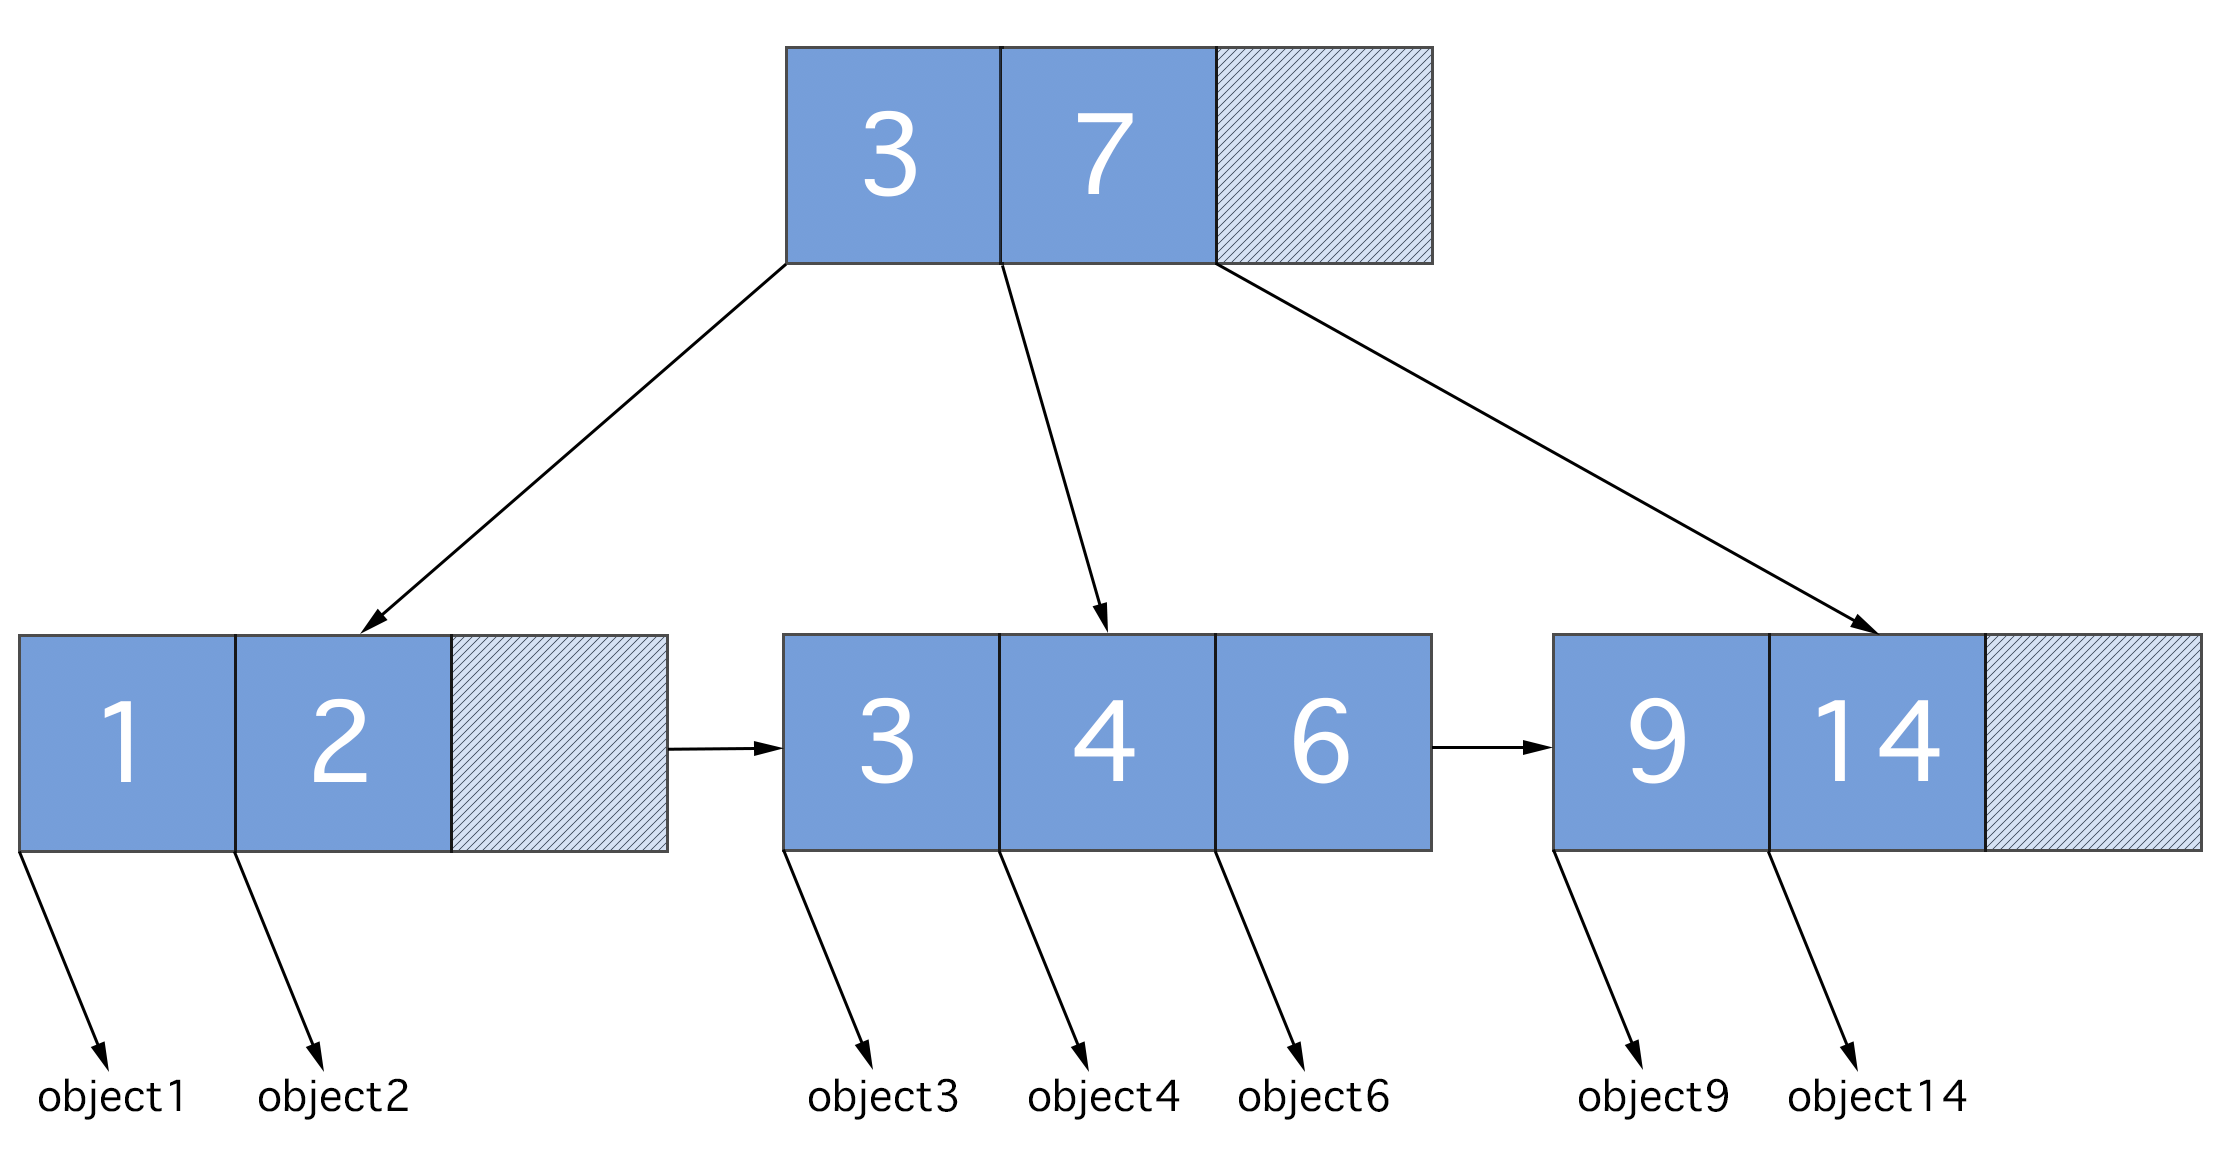
\includegraphics[width=\textwidth,height=\textheight,keepaspectratio]{img/b+tree.png}
    \caption[The architecture of the system]{ The architecture of the system. The
      \textit{Viper IDE} and \textit{Viper Debugger} boxes denote, respectively,
      the main Viper extension and the new debugger extension. They both interact,
      independently, with Visual Studio Code. Viper Server is responsible for
      running the verification backends.}
    \label{fig:b+tree}
\end{figure}

[add characteristics from wiki?]

\section{Specific implementation}\label{sec:specific-implementation}
For our application, the basic B+tree needs to have some extra characteristics added to it. 

First of all, each node (root, inner and leaf nodes) will store statistics based on the operations performed. In particular, each node will have two counters, one for read and one for write operations, for each group in the system. Therefore, if we have three groups, each node will have six counters. The statistics are updated from the root up to the node that handles the item accessed.

[put picture that shows statistic update]
\begin{figure}[htb]
  \centering
  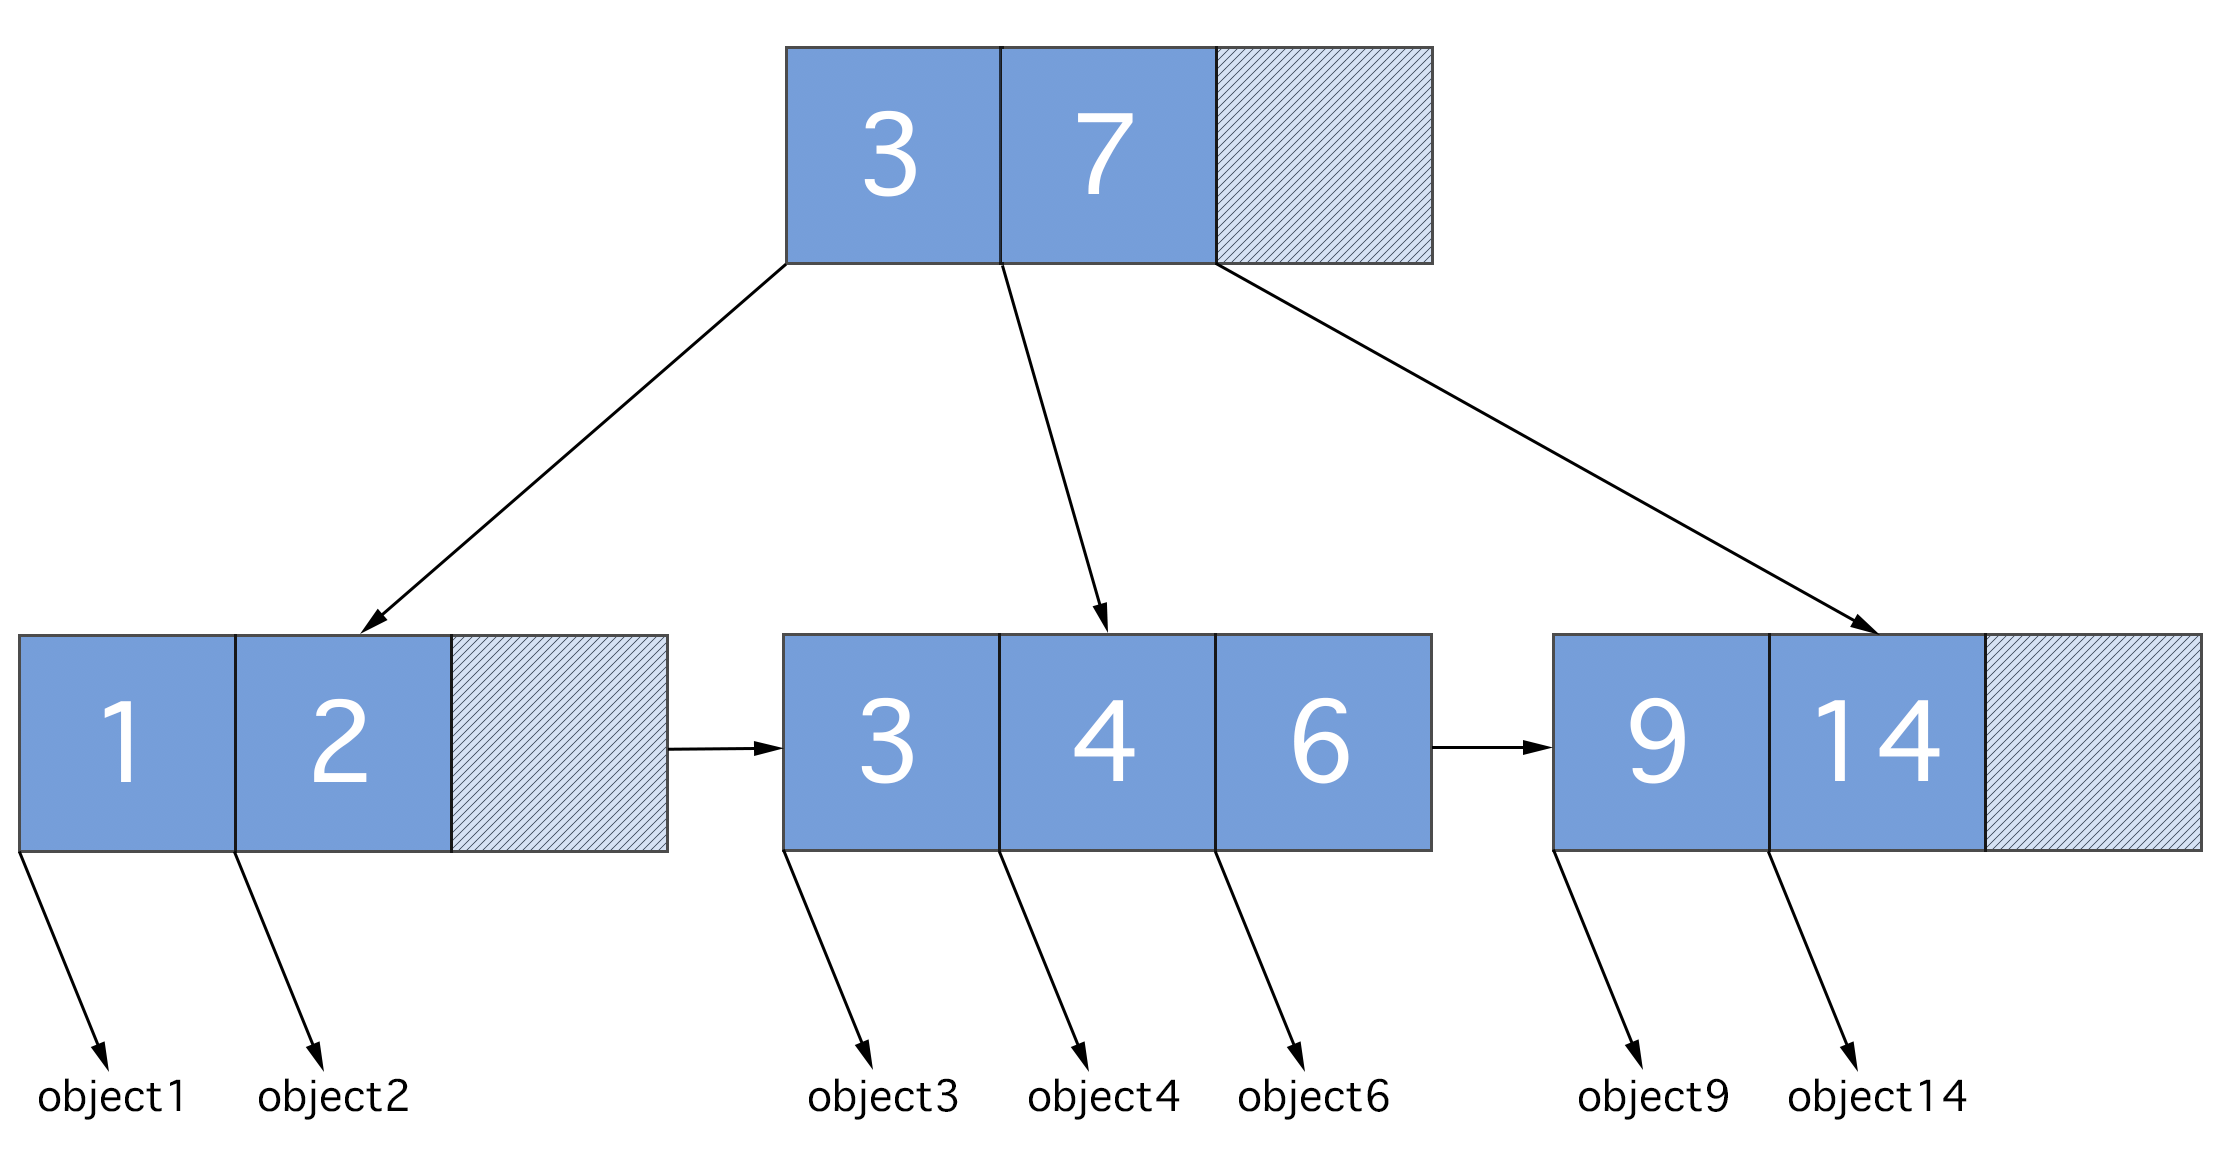
\includegraphics[width=\textwidth,height=\textheight,keepaspectratio]{img/b+tree.png}
  \caption[The architecture of the system]{ The architecture of the system. The
    \textit{Viper IDE} and \textit{Viper Debugger} boxes denote, respectively,
    the main Viper extension and the new debugger extension. They both interact,
    independently, with Visual Studio Code. Viper Server is responsible for
    running the verification backends.}
  \label{fig:b+tree}
\end{figure}

These statistics will be used as workload when the repartition will be executed. Once the repartition is performed, the statistics will be updated with the formula:
$$ current\_statistics = \alpha \cdot old\_statistics + (1-\alpha) \cdot new\_statistics $$
Where the old statistics are the ones gathered until the past repartition, and the new statistics are the ones between the past repartition and the current one.
[put picture that shows which are old and which are new?]
\begin{figure}[htb]
  \centering
  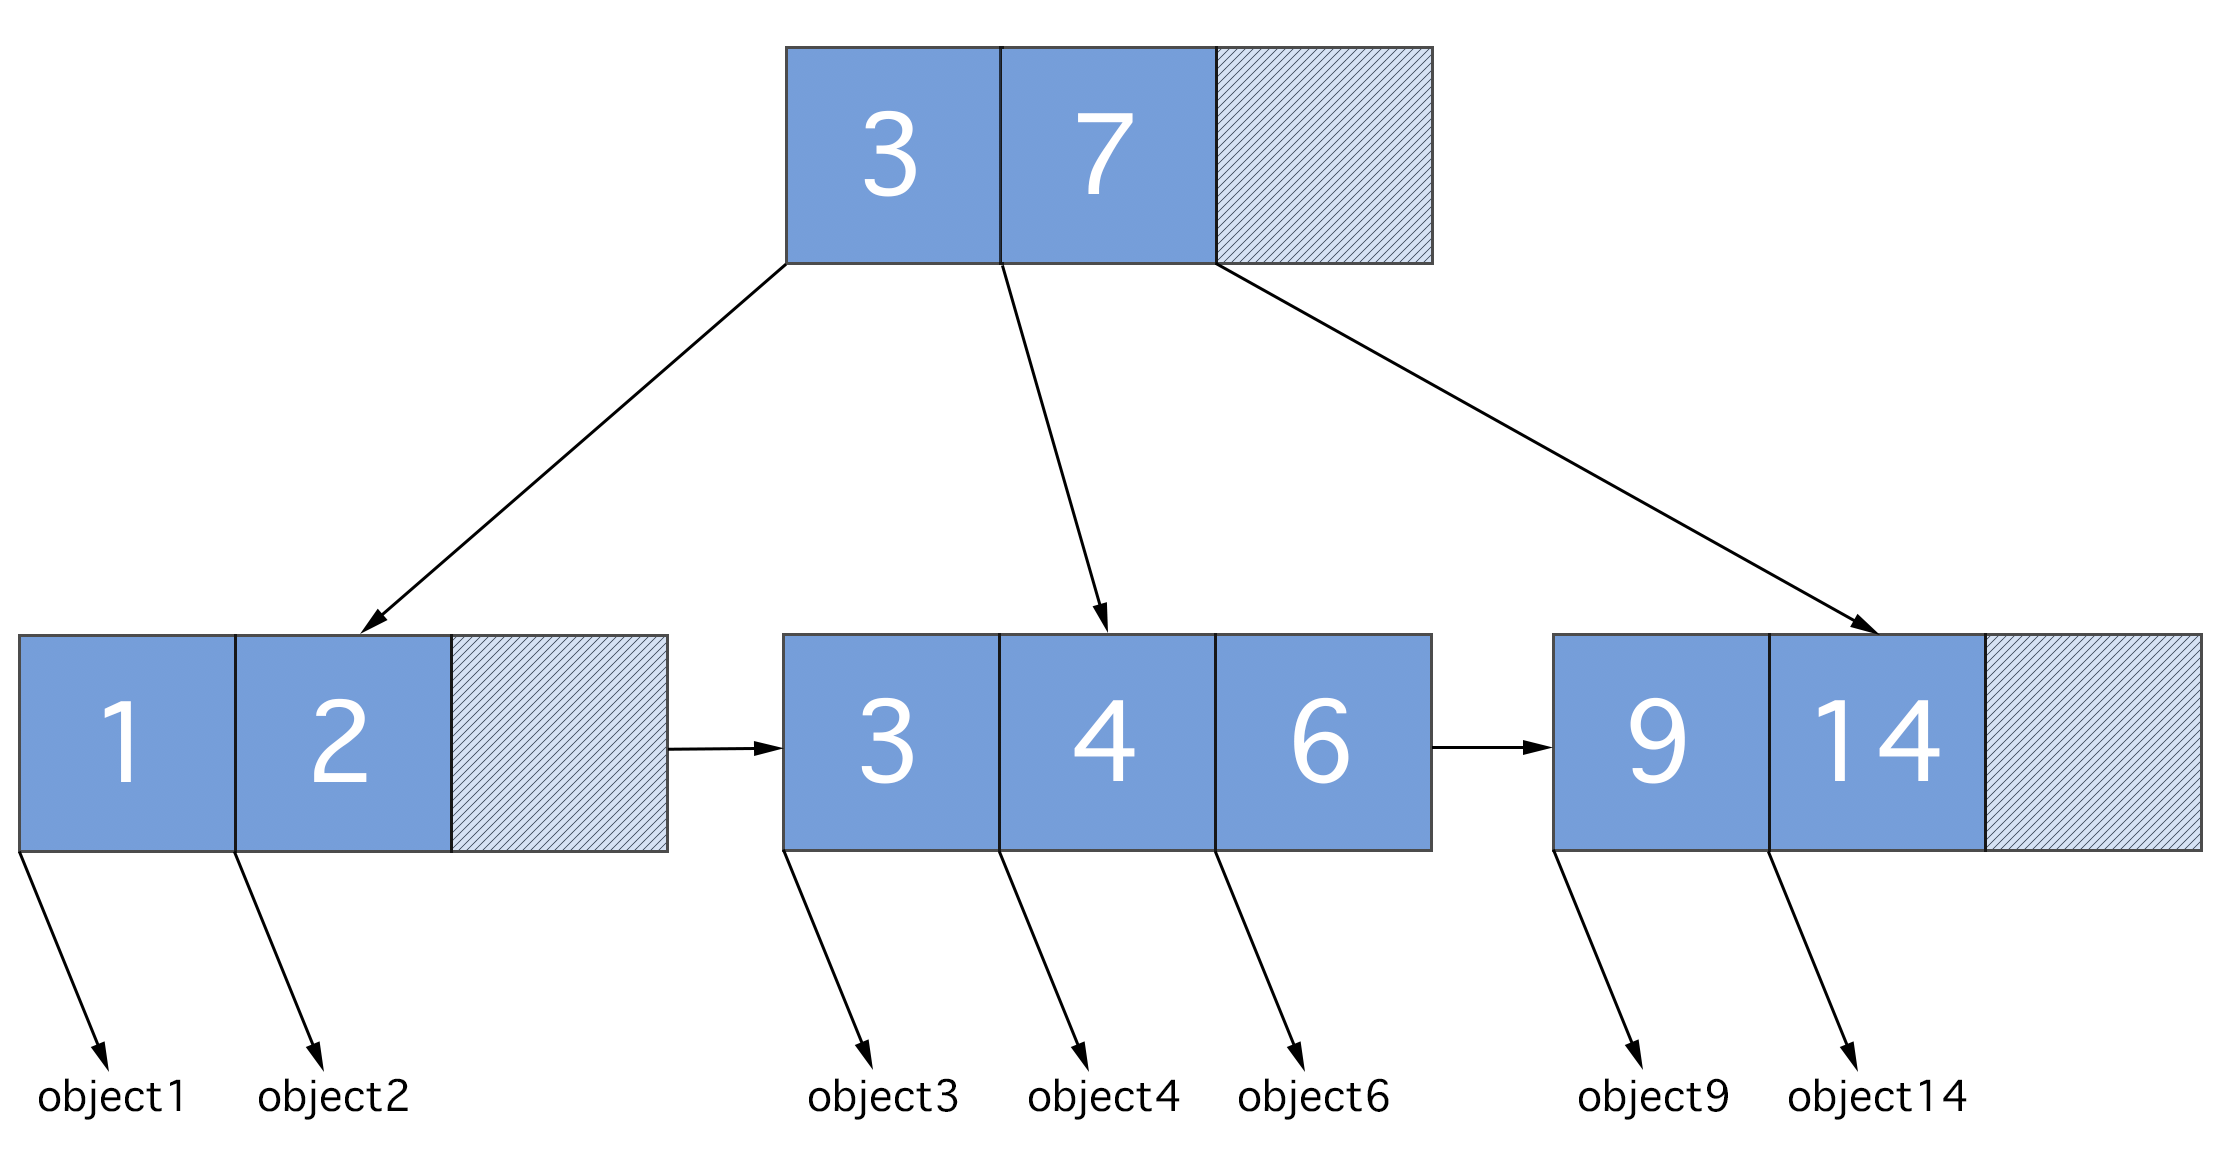
\includegraphics[width=\textwidth,height=\textheight,keepaspectratio]{img/b+tree.png}
  \caption[The architecture of the system]{ The architecture of the system. The
    \textit{Viper IDE} and \textit{Viper Debugger} boxes denote, respectively,
    the main Viper extension and the new debugger extension. They both interact,
    independently, with Visual Studio Code. Viper Server is responsible for
    running the verification backends.}
  \label{fig:b+tree}
\end{figure}

Furthermore, whenever a node is full and it has to split, its statistics are halved evenly between the two nodes. This is because we don't know which statistics correspond to which data item in particular, but we can assume that there is a decent chance that keys that are close to each others will have similar statistics.

The second thing that we need to store in the nodes of our B+tree are the partitions. In particular, we need to store both the partitions that take care of each node, and the preferred partition in case there are multiple partitions to choose from. Initially, each new node will be replicated to all partitions of the system. This is to make sure that all clients will initially have the same availability of the data items. Once we issue a repartition, the algorithm will calculate the optimal partitions for each node based on the workload. These optimal repartition will be used to know which replicas to involve in the following operation on each object, until the next repartition. 

If a node splits, the new node will inherit the partitions from the full node. This is again a heuristic, based on the high likelihood that close keys will have similar accesses.


\section{Optimization approaches}\label{sec:optimization-approaches}
In this section I will first explain in detail how we calculate the optimal group assignment of data objects to the partitions based on the workload. I will then go over the various approaches that were attempted to improve the repartition optimization. 

\subsection{Optimal partitions algorithm}\label{sec:optimal-partitions-algorithm} 
!!! fa un po' schifo
The simplest algorithm to implement is the one that compares all the possible combinations of partitions and picks the best one. While this algorithm will give the optimal assignments for minimum average latency for a certain workload, it is also the one that takes the longer amount of time. We will use the performance of this algorithm as a [starting point?] to compare our later algorithms with.

The algorithm goes top to bottom and it calculates the partitions for each node. For each node, we get the workload, that may looks as follows:

\begin{table}[htb]
  \centering
  \begin{tabular}{l l l l}
    \hline
    & \textbf{Group 1} & \textbf{Group 2} & \textbf{Group 3} \\
    \hline
    \textbf{Reads} & 150 & 37 & 540 \\
    \textbf{Writes} & 32 & 10 & 93 \\
    \hline
  \end{tabular}
  \caption{Example of a possible workload of a node in a case with 3 groups. The node counts the number of read and write operations received from each group, to be used for the repartition algorithm.}\label{tab:workload-example}
\end{table}

We then load a graph that represents the geographic placements of the various replicas, where the cost of the edges is the estimated average Round Trip Time required to send a message.
[put a pic with a graph]

We then proceed by looping over all possible combinations of partitions, where a partition can be taken or not taken. Obviously, at least one partition has to be taken. In the case of 3 groups, we would have to consider $2^3 -1 = 7$ combinations: $001, 010, 100, 011, 101, 110, 111$, where 1 and 0 mean that the object will be or will not be assigned to that specific replica, respectively.

Given the number of reads and writes for each group, and the current groups to which we're replicating this object, we multiply the number of reads by the latency with the closest replica that would have this object. For writes, we have to add the latency of all the replicas that have this object, since the operation is going to modify the data item.

Also note that the result depends on the latency that we are currently considering: for example, if we're doing the calculations from the point of view of a replica that will not have this object, each read will have to go to a different replica; therefore we have to consider the costs from the point of view of all the replicas.

Once we have gone over all the combinations, we pick the one with the lowest cost, and we move onto the next object.

\subsection{fixed-size buckets}\label{sec:fixed-size buckets}
One of the ideas to improve the performance of the repartition is to try to reduce the number of nodes that we have to do the calculations for. Since the tree is divided in levels, the idea is to group nodes of different levels in what we call \emph{buckets} and do an aggregated calculation of the optimal partition assignment for the whole bucket. An example of a bucket can be seen in figure [sotto]. As a reminder, whenever a operation is performend on an object, the statistics of the tree are updated along the whole path from the root to the node that handles this object. This means that in general, the parent node will have the aggregated statistics for all its children nodes (this may not always be the exact case when the parent node splits, but this is not particularly frequent, and even when it happens the statistics of the split nodes are good approximations of the real statistics).

There are also multiple ways to group things in the case where we have an odd number of levels. Since we're using buckets of two levels, we could either allow the root node to be a bucket of 1 level, or let the leaves be buckets of 1 level. Or, we could have the root be the only bucket to be allowed to have 3 levels. [put pic] The first one would not reduce the number of saved calculations by much, since most nodes are on level 0; the other two options make virtually no difference, as they only affect the level with the least amount of nodes. We decided to go with the second option, allowing the root node to be in a bucket of its own in case of odd levels.

It is also important to remember that this improvement affects only the number of objects, not the groups; therefore, in the case where we have $n$ objects and $m$ groups, this would improve on the linear number of objects $n$ but it would not affect the number of combinations, which grows as $2^m$.

In general, given a branching factor of $b$ of and objects $n$, the number of calculations we would be doing would be around $\approx\cfrac{n}{b}$ as the tree grows, since we are approximating all the calculations at level 0, which in a big tree is by far the level with the most nodes.

[performance?]
[specify how many calculations we are saving?]

[pic of grouped levels]
\begin{figure}[htb]
  \centering
  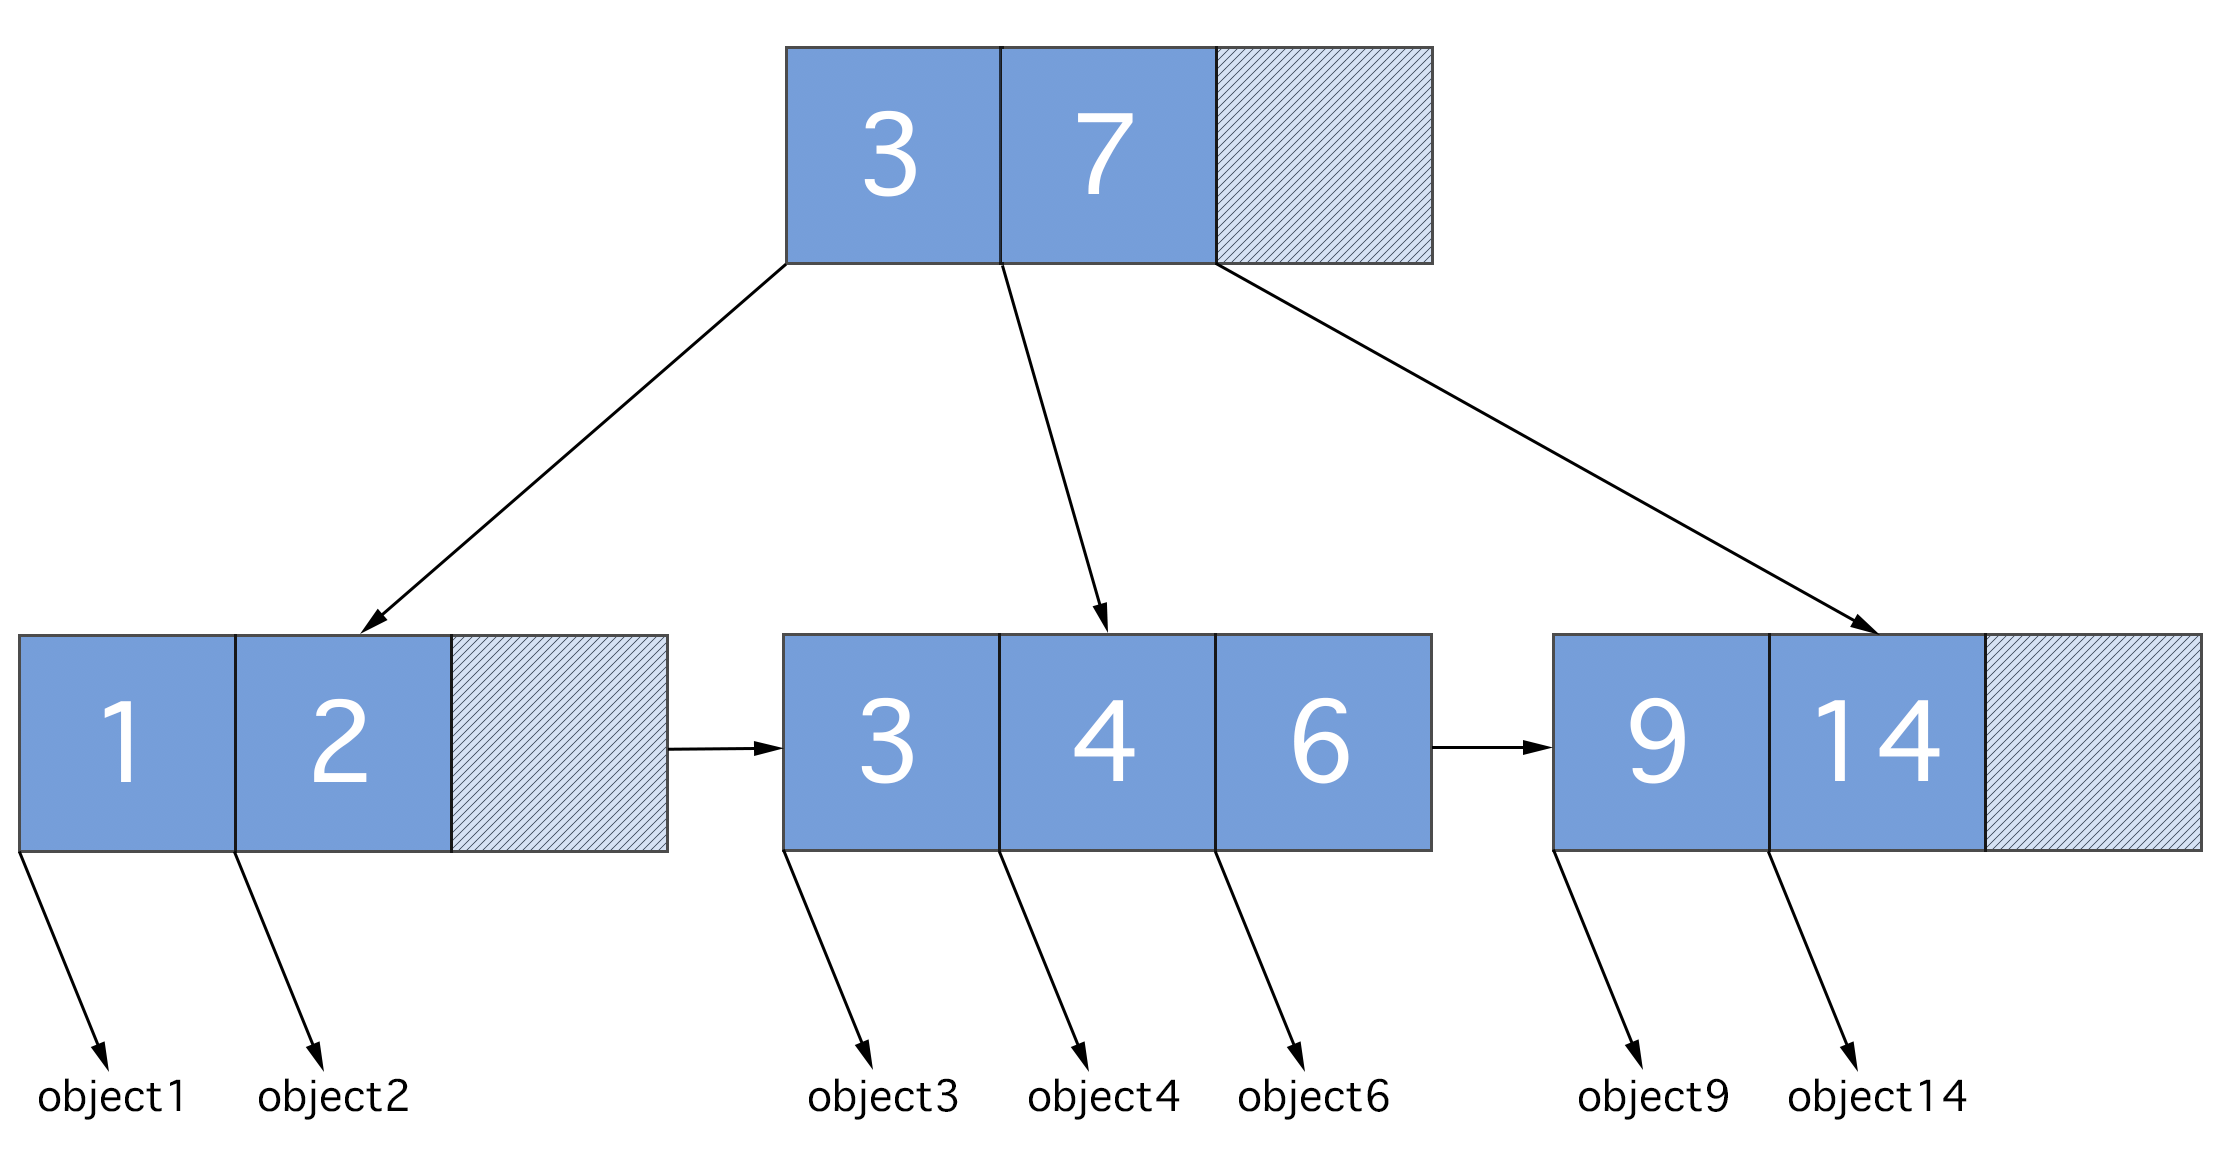
\includegraphics[width=\textwidth,height=\textheight,keepaspectratio]{img/b+tree.png}
  \caption[The architecture of the system]{ The architecture of the system. The
    \textit{Viper IDE} and \textit{Viper Debugger} boxes denote, respectively,
    the main Viper extension and the new debugger extension. They both interact,
    independently, with Visual Studio Code. Viper Server is responsible for
    running the verification backends.}
  \label{fig:b+tree}
\end{figure}

\subsection{variable-size buckets}\label{sec:variable-size buckets}
The idea of the fixed-size buckets is interesting, as it greatly reduces the number of nodes we have to account for, but it also approximates the problem too much. Reducing the branching factor would not be a solution, as it would just increase the number of nodes once more, and because the high branching factor is one of the main reasons to use a B+tree. 

An alternative approach is to to have a variable, or dynamic, size of buckets. The idea is to group in two or more levels the nodes that have a low amount of statistics, and instead do the optimal calculations for the nodes with many operations associated to them. The idea is that approximating the nodes with few operations would not hinder the performance by much, as the object associated to those nodes will not be accessed often by the clients, while instead the objects that are used often will have their optimal partitions.

It is also more likely for the nodes towards the leaves to be approximated, since the parents will have the aggregated statistics of all their children.

One challenge of the variable-size buckets approach is to figure out when it is worth doing the full calculations and when it is better to group in buckets. In the case where the operations are evenly distributed among all children of a node, we will have that the statistics of a child node will be around $\cfrac{1}{b}$ of the parent node. Then, we could say that if, for example, a child node has less than $\cfrac{1}{b^2}$[random number], then we should place it in a bucket; but finding the right number depends on many variables and on the system at hand, therefore finding a good value would have to be fine-tuned depending on the application.

[pic of grouped levels]
\begin{figure}[htb]
  \centering
  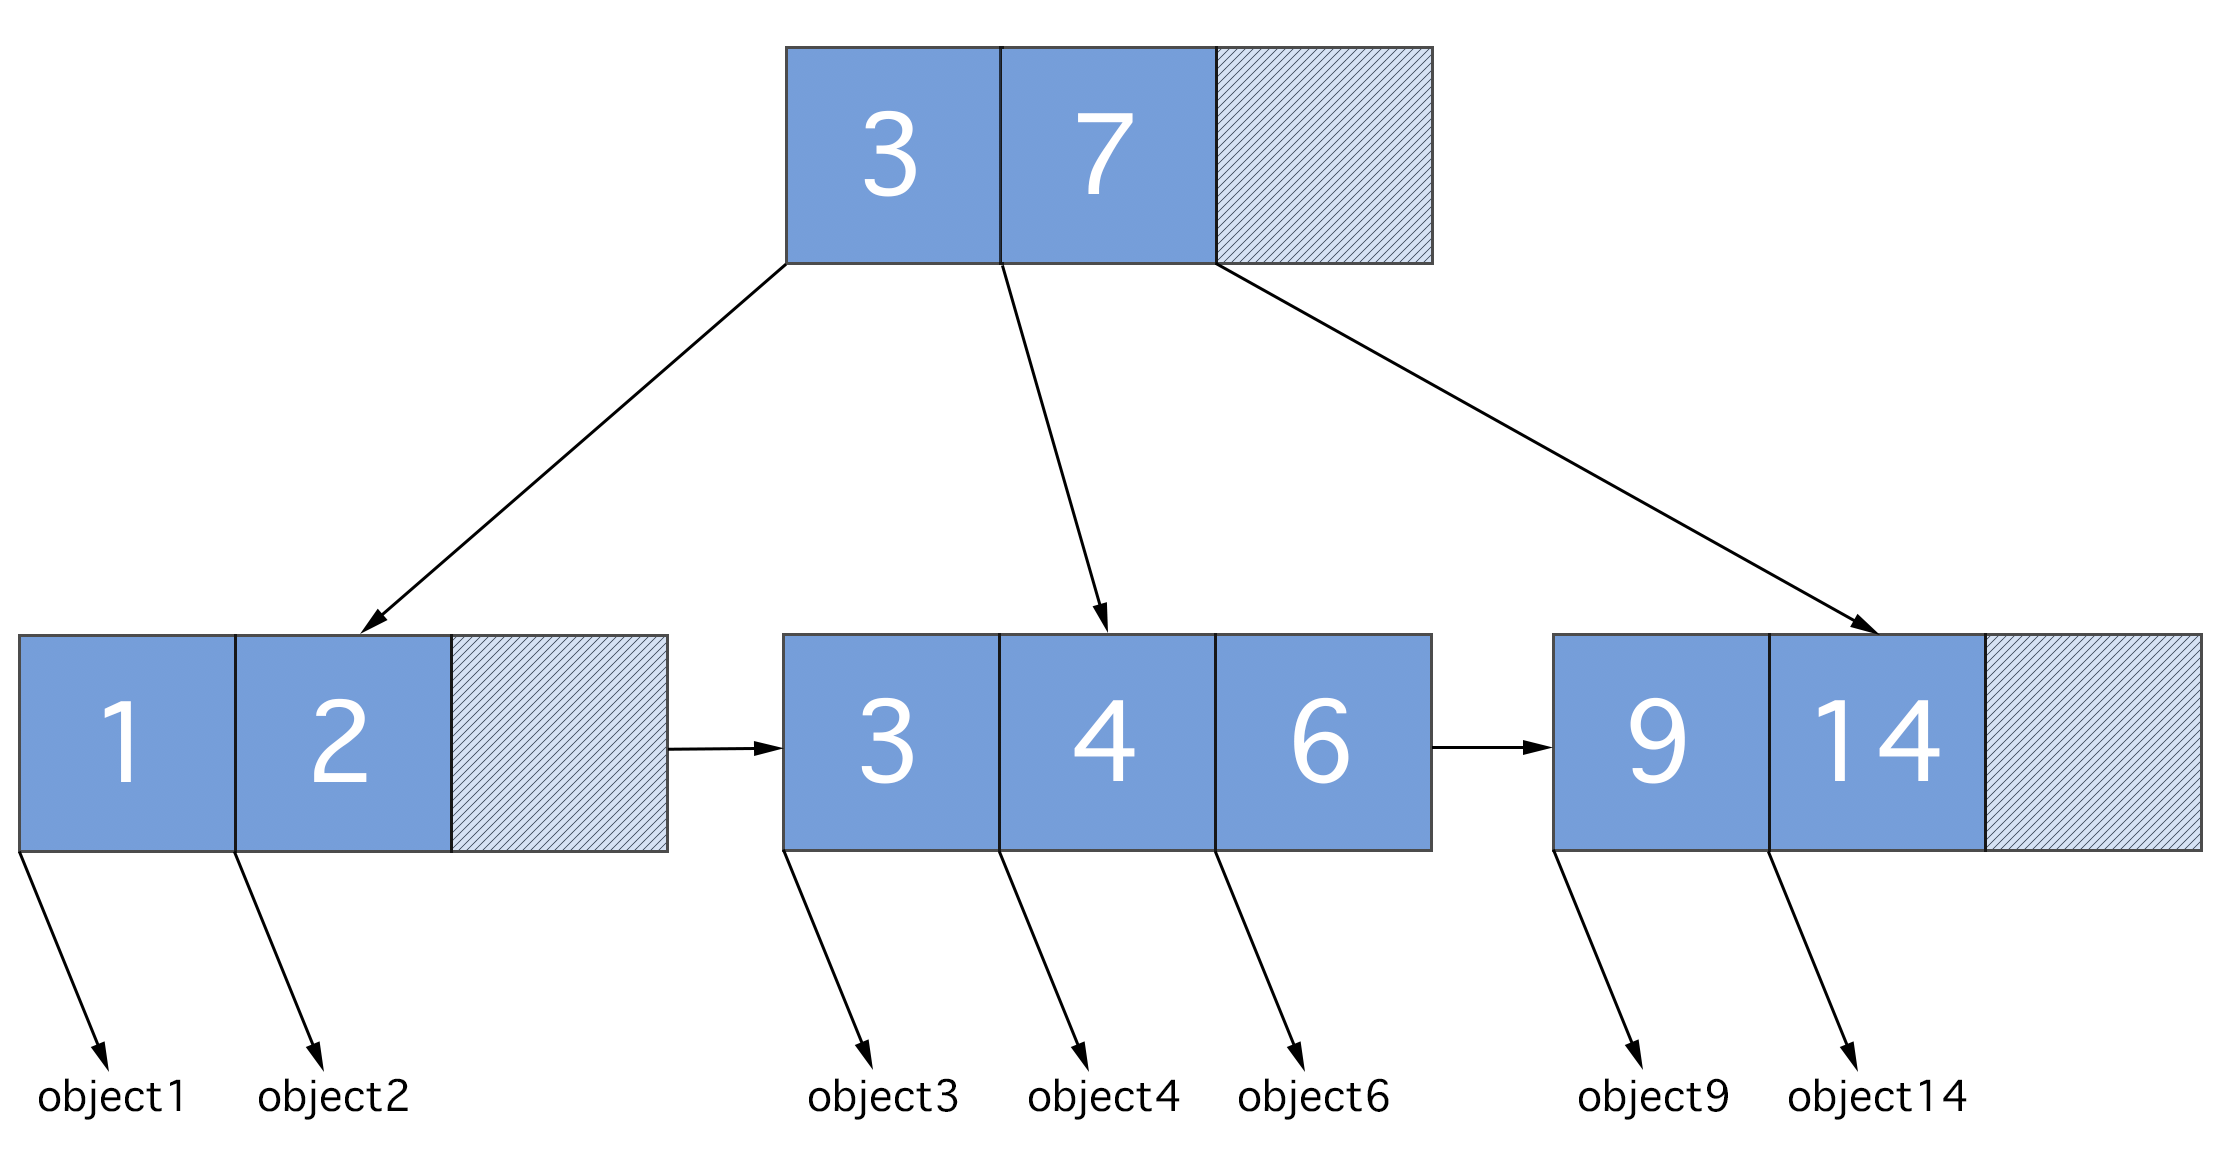
\includegraphics[width=\textwidth,height=\textheight,keepaspectratio]{img/b+tree.png}
  \caption[The architecture of the system]{ The architecture of the system. The
    \textit{Viper IDE} and \textit{Viper Debugger} boxes denote, respectively,
    the main Viper extension and the new debugger extension. They both interact,
    independently, with Visual Studio Code. Viper Server is responsible for
    running the verification backends.}
  \label{fig:b+tree}
\end{figure}

\subsection{hot groups}\label{sec:hot-groups}
Another option is to try to reduce the number of combinations that we have to consider for each node. Since the complexity grows exponentially with the number of groups, if we're able to discard some combinations before we calculated their actual cost, then we should have a greater improvement compared to the optimizations that reduce the number of nodes.

One idea to do this is as follows: given a workload, there is a chance that one or more groups will have fewer operations on the current node compared to other groups. Then, there is a big chance that the final partition assignment wouldn't replicate the objects to the partition/group with fewer operations, since the gain of replicating the object to said partition would be less than the added cost of it.

The gain/cost of replicating to a group with few operations also depends on the ratio between read/write operations, obviously: with many reads we would want to assign the object to all groups, while with many writes we would want to reduce the number of group assignments, as with every write we would have to coordinate between all groups involved. In general, though, such a system is better suited for applications with more reads than writes, therefore our assumption of discarding groups with few operations still holds.

The way to implement this is fairly simple: with the workload at hand, we find the group or groups with the highest number of operations (the ``hot groups''). Then, when we're going through all the possible combinations of groups, we discard those that would assign the object to groups with much lower operations than the hot groups. As before, finding the ideal threshold is no easy task; a higher threshold would discard more combinations making the computations faster but possibly lose a lot of accuracy, while a lower threshold might only skip very few combinations giving us very small performance gains. 


\begin{table}[htb]
  \centering
  \begin{tabular}{l l l l}
    \hline
    & \textbf{Group 1} & \textbf{Group 2} & \textbf{Group 3} \\
    \hline
    \textbf{Reads} & 150 & 37 & 540 \\
    \textbf{Writes} & 32 & 10 & 93 \\
    \hline
  \end{tabular}
  \caption{Example of a possible workload of a node in a case with 3 groups. In this case, group 3 would be the hot group, since it is the node with more total operations. Depending on the threshold, we could discard only group 2 or both group 1 and 2 from the list of possible assignment combinations; this would reduce the number of combinations for this node from 7 to 3 or 1, respectively.}\label{tab:workload-example}
\end{table}

[logic behind it, with a picture/table to show workloads and which group to discard]

[difficulty of choosing threshold]

\subsection{LRU caching}\label{sec:lru-caching}
[maybe start with a complete description, then go bit by bit]
This method makes use of two important characteristics that can be observed in our applications, which allow us to use a different type of approach to improve the performance of the repartition.

\subsubsection{First key}\label{sec:first-key}
The first one is that as long as the geographic structure of our whole system does not change, then the partition assignment will always be the same whenever the statistics of the nodes are the same. The geographic information is stored in the graph that contains the latencies between the various replicas in the respective regions; this won't change while our system is running, and in a real world application too it shouldn't change often, as it would mean that we either change completely a server or that we move them around. 

This means that we may end up doing the same calculations multiple times, getting the same results each time. Therefore, we should instead store the results, so that the second time we face the same workload we can just load the result. 

Since we want to be able to load the results quickly, the first data structure that comes to mind would be some kind of map, so that we can get them in $a\approx O(1)$ time. This spawn two issues.

How do we define the key? we know that simply using the workload as the key would be enough, but we could ideally have an infinite number of different loads, since the statistics are unbounded, and since we can have a varying amount of groups, the amount of combinations would grow even larger. Also, workloads that are multiples of each others would give us the same assignment of partition, meaning that we would have multiple keys for the same values for no reason.

These two issues could lead us to having a data structure that grows to an uncontrollable size.

What we can do instead is to encode the workload in a new type of key. Remember that for each group we have a value for reads and writes. For each group, we will calculate the read write/ratio and the update ratio. The read/write ratio is just the amout of total operations for each group compared to the total number of operations for the whole node. For example, with the example workload of table[put number], we would have read write ratios of:
$$ 11/14, 3/14 $$

Then we calculate the update ratio for each group, which is the ratio between reads and writes for said group. Again, with the workload of table[table] we would get:
$$1/11 2/3 $$

The ratios can then be approximated to different precisions, depending on our needs. If we normalize them from 0 to 9 we would have a far smaller data structure, but it would also be a quite big approximation. 0 to 99 would give us an acceptable approximation without giving us humongous keys, as long as we don't have a lot of groups. 

Finally, we get the key for this workload by concatenating the values:
$$ K = RW_1 U_1 RW_2 U_2 $$

Our final key for table[table] would be, if we use 0-99 values:
$$ K = $$

\begin{table}[htb]
  \centering
  \begin{tabular}{l l l l}
    \hline
    & \textbf{Group 1} & \textbf{Group 2} & \textbf{Group 3} \\
    \hline
    \textbf{Reads} & 150 & 37 & 540 \\
    \textbf{Writes} & 32 & 10 & 93 \\
    \hline
  \end{tabular}
  \caption{Example of a possible workload of a node in a case with 3 groups. In this case, group 3 would be the hot group, since it is the node with more total operations. Depending on the threshold, we could discard only group 2 or both group 1 and 2 from the list of possible assignment combinations; this would reduce the number of combinations for this node from 7 to 3 or 1, respectively.}\label{tab:workload-example}
\end{table}


[is there another issue? forgot]

\subsubsection{Second-key}\label{sec:second-key}

Our workload to key encoding now gives us a fair improvement, allowing us to discard workloads that would be duplicates and also limit the number of possible entries by normalizing them to an interval. The issue of having too many keys is still present, though: let's say we have 5 groups and we use 0-99 values, we would have 0-9999 combinations for each group, therefore having $10^{20}$ keys, for an example that is not even that big. We then have to further limit the number of keys. 

The hindsight that can help us improve on what we have is that many of those keys will never be used; for example, the key with all 0s does not represent any workload we could have. Also, even a key with a possible workload could be very unlikely and rare case, and therefore we could just not store it and just do the recalculation the few times we do encounter such a workload. 

A possible way to exploit this is by implementing a sort of Least Recently Used (LRU) approach: we can limit the maximum number of keys that we store in our data structure, and once we want to add a new key but the limit has been reached, we evict the least recently used key and we add the new one. We still don't want to degrade the efficiency of the data structure: we still want to be able to retrieve and add a key in amortized constant time.

[explanation of LRU, how the list works, and so on]
[pretty picture of LRU]
\begin{figure}[htb]
  \centering
  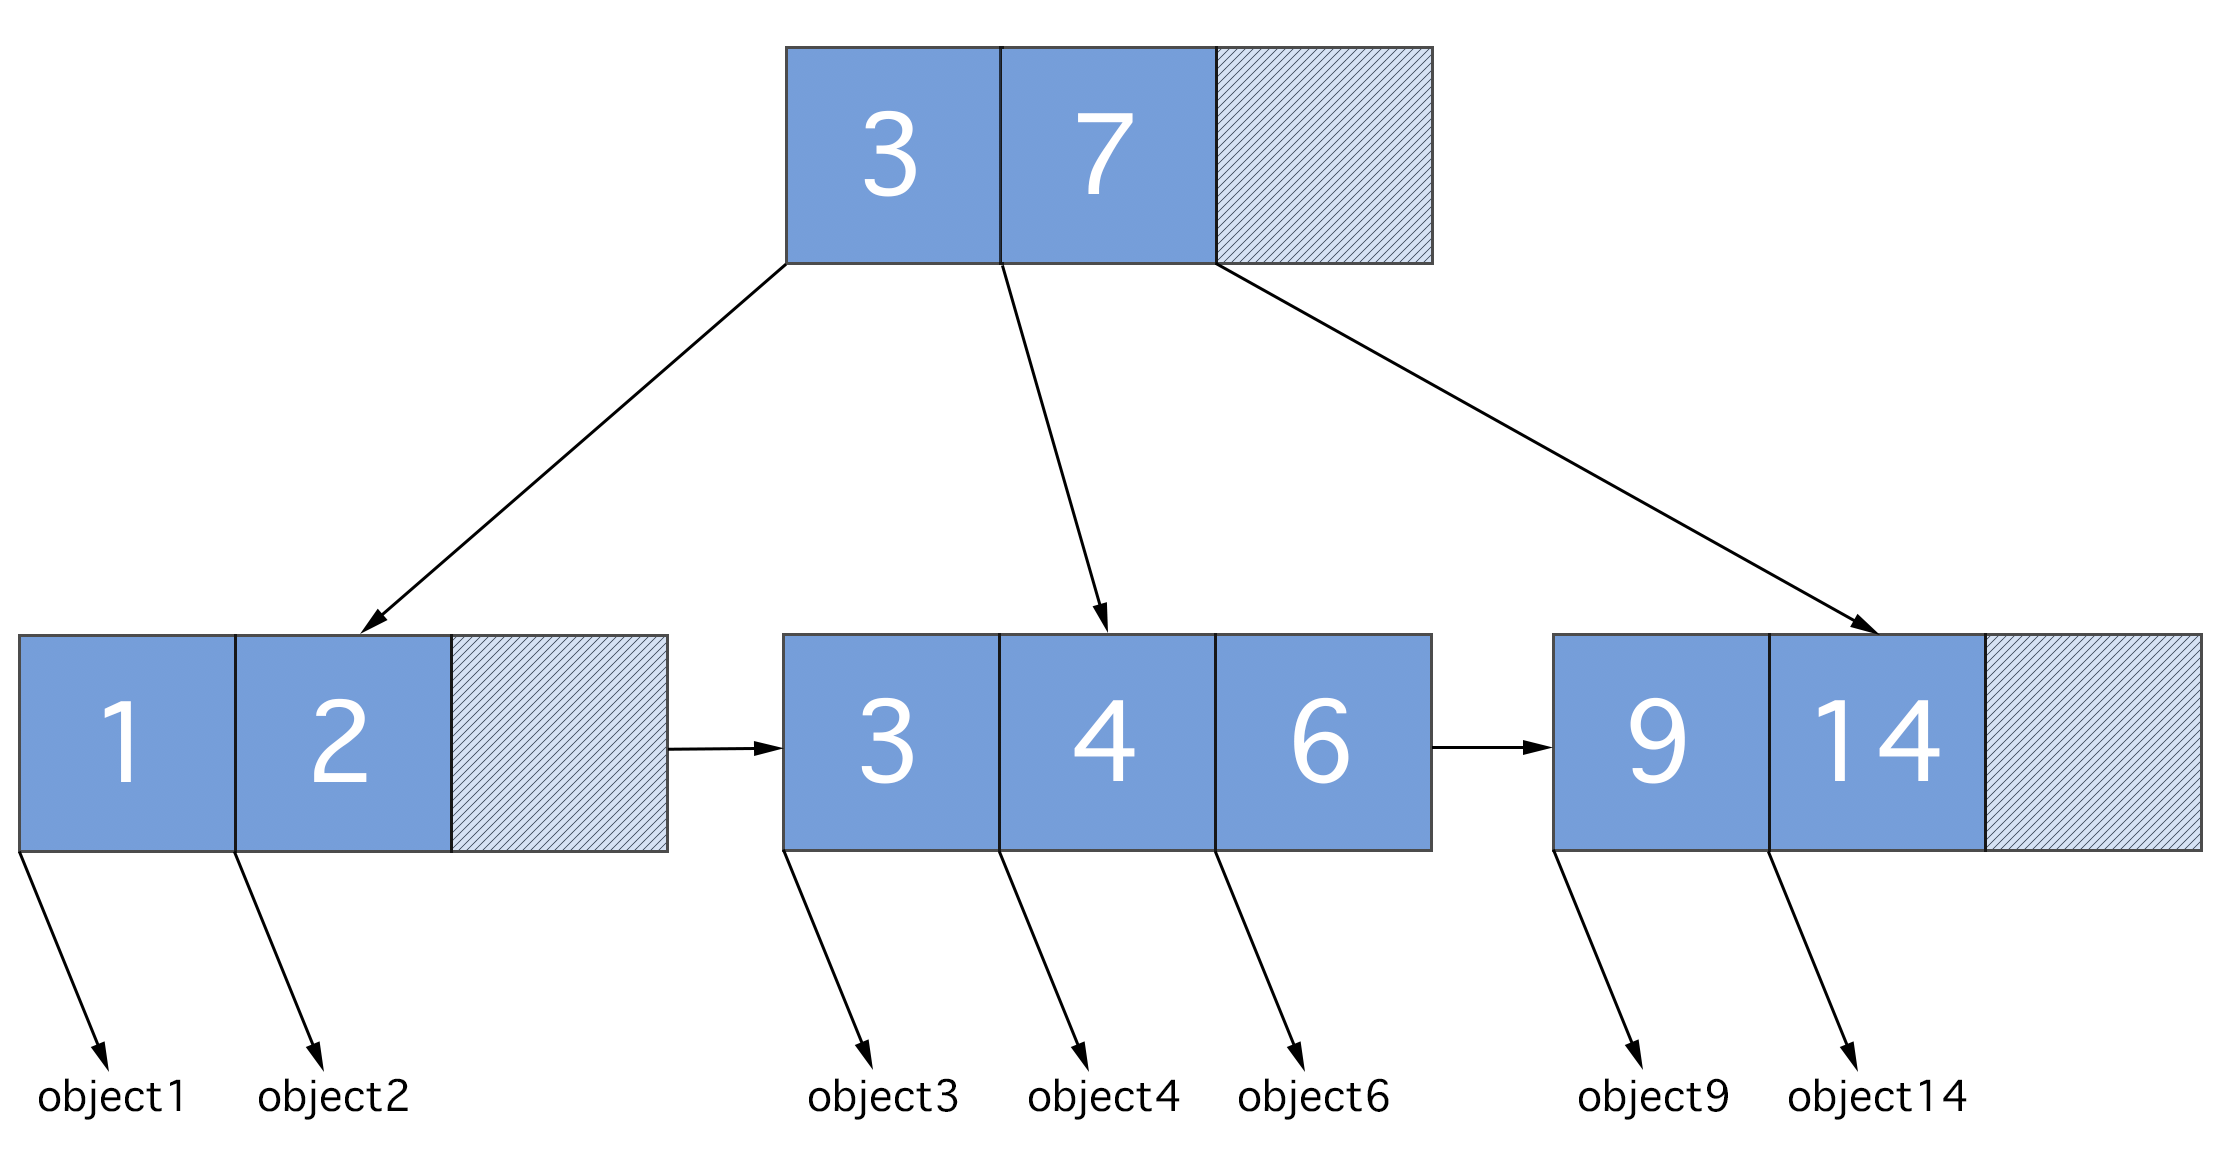
\includegraphics[width=\textwidth,height=\textheight,keepaspectratio]{img/b+tree.png}
  \caption[The architecture of the system]{ The architecture of the system. The
    \textit{Viper IDE} and \textit{Viper Debugger} boxes denote, respectively,
    the main Viper extension and the new debugger extension. They both interact,
    independently, with Visual Studio Code. Viper Server is responsible for
    running the verification backends.}
  \label{fig:b+tree}
\end{figure}

[warming up, pre warm-up]


\section{Optimization tests}\label{sec:optimization-tests}

for the types of optimizations with variables, say what they were set to, such as 0.1 for LRU

\section{GeoPaxos tests}\label{sec:geopaxos-tests}

\subsection{tests-setup}\label{sec:tests-setup}

[explain types of clients, show skew, type of distribution, loads]
[put structure, with replicas, geo-locations, cite geopaxos for latencies]

[say how the clients act, put a skew graph, different types of clients, repartitino timings...]